\chapter[Projekt konstrukcji sonaru oraz protokoły komunikacji]{Projekt konstrukcji sonaru oraz protokoły komunikacji}

\label{konstrukcja}

Tutaj powinien być opis części mechanicznej, schematy elektroniczne,
opis protokołu komunikacji wraz z opisem implementacji (w protokole)
listy poleceń.
Opis funkcjonalności, które będą oferowane przez aplikację
oraz sposob przetwarzania danych pomiarowych i ich reprezentacji.

\section{Komunikacja}

\subsection{Wybór protokołu}

Wybrany został protokół UART, ze wględu na to, że płytka deweloperska STM32 NUCLEO-L476RG 
z której skorzystano w projekcie posiada wbudowany konwerter UART$\rightarrow$~USB, 
co pozwala na skomunikowanie mikrokontrolera z komputerem bez dodatkowego sprzętu.

\subsection{Komputer \textrightarrow{} sonar}
Użytkownik systemu może wysłać z komputera instrukcję do wywołania całej sekwencji działania urządzenia. 
Ramka danych zaczyna się znakiem specjalnym ułatwiającym rozpoznanie wiadomości, 
następnie musi zostać podany numer komendy informujący sonar jaką czynność powienien wykonać, 
parametry określające warunki tej czynności, a na koniec suma kontrolna wiadomości.

\begin{figure}[!ht] %data in
    \centering
    \begin{tikztimingtable}[timing/wscale=4]
        \tikzset{% Environment Config
            timing/dslope=0.1,
            timing/.style={x=5ex,y=2ex},
            x=5ex,
            timing/rowdist=3ex,
            timing/name/.style={font=\sffamily\scriptsize},
            timing/d/text/.style={font=\sffamily\tiny},
        }
        \textcolor{black}{Instruction} & [black]
            Z 1D{X}  1D{CMD\_ ID} 1D{PAR1} 1D{PAR2} 1D{PAR3}   1D{CRC}  \\ %
        \textcolor{black}{Bytes} & [black]
            Z 1D{1}  1D{1}        1D{1}    1D{1}    1D{4}      1D{4}    \\ %
        %
        % there must NOT be an uncommented line before \extracode!
        %
        \extracode
            \tablerules
        %%  \tablegrid
        
        \begin{pgfonlayer}{background}
            \begin{scope}[semitransparent ,semithick]
                %\vertlines[darkgray,dotted]{1.0,3.0,...,23.0}
                \vertlines[gray,dotted]{4.0,8.0,...,\twidth}
            \end{scope}
        \end{pgfonlayer}
        \end{tikztimingtable}
        \caption{Ramka danych przychodzących}
        \label{fig:datain}
    \end{figure}
    \todo{zrobić ładniejszą ramkę}

% \begin{figure}[!h]
%     \centering
%     \begin{tikztimingtable}[timing/wscale=4]
%         \tikzset{% Environment Config
%             timing/dslope=0.1,
%             timing/.style={x=5ex,y=2ex},
%             x=5ex,
%             timing/rowdist=3ex,
%             timing/name/.style={font=\sffamily\scriptsize},
%             timing/d/text/.style={font=\sffamily\tiny},
%         }
%         \busref*{FRAME}      & 2u 1d 2d 2u \\
%         \textcolor{black}{Instruction} & [black]
%             Z 1D{X}  1D{COM\_ID} 1D{CRC}    \\ %
%         \textcolor{black}{Bytes} & [black]
%             Z 1D{1}  1D{1}       1D{4}      \\ %
%         %
%         % there must NOT be an uncommented line before \extracode!
%         %
%         \extracode
%             \tablerules
%         %%  \tablegrid
        
%         \begin{pgfonlayer}{background}
%             \begin{scope}[semitransparent ,semithick]
%                 %\vertlines[darkgray,dotted]{1.0,3.0,...,23.0}
%                 \vertlines[gray,dotted]{4.0,8.0,...,\twidth}
%             \end{scope}
%         \end{pgfonlayer}
%         \end{tikztimingtable}
%     \end{figure}
    

\subsection{Sonar \textrightarrow{} komputer}

Sonar w odpowiedzi na instrukcję wysyła ramkę danych która również zaczyna się znakiem specjalnym, 
następnie podawany jest numer komendy na którą sonar odpowiada, status wykonania, dane pomiarowe oraz suma kontrolna.
\begin{figure}[!ht] %data out
\centering
\begin{tikztimingtable}[timing/wscale=4]
    \tikzset{% Environment Config
        timing/dslope=0.1,
        timing/.style={x=5ex,y=2ex},
        x=5ex,
        timing/rowdist=3ex,
        timing/name/.style={font=\sffamily\scriptsize},
        timing/d/text/.style={font=\sffamily\tiny},
    }
    \textcolor{black}{Instruction} & [black]
        Z 1D{X}  1D{ANS\_ID} 1D{STATUS} 1D{ZC\_NUM} 1D{TCL} 1D{D11} 1D{...} 1D{D33}  1D{CRC}  \\ %
    \textcolor{black}{Bytes} & [black]
        Z 1D{1}  1D{1}       1D{1}      1D{1}       1D{4}   1D{4}   1D{...} 1D{4}    1D{4}    \\ %
    %
    % there must NOT be an uncommented line before \extracode!
    %
    \extracode
        \tablerules
    %%  \tablegrid
    
    \begin{pgfonlayer}{background}
        \begin{scope}[semitransparent ,semithick]
            %\vertlines[darkgray,dotted]{1.0,3.0,...,23.0}
            \vertlines[gray,dotted]{4.0,8.0,...,\twidth}
        \end{scope}
    \end{pgfonlayer}
    \end{tikztimingtable}
    \caption{Ramka danych wychodzących}
    \label{fig:dataout}
\end{figure}
\todo{zrobić ładniejszą ramkę}


\section{Elektronika}
Projekt bazuje na autorskiej płytce z obwodem drukowanym, który został zaprojektowany przy pomocy 
otwartoźródłowego narzędzia do projektowania elektroniki ,,KiCad" \cite{kicad}.

\subsection{Zasilanie}
Całe urządzenie zasilane jest z portu USB komputera, które jednocześnie służy do komunikacji. 
Przewód jest podłączony bezpośrednio do płytki deweloperskiej Nucleo, 
a zaprojektowane na cele pracy dyplomowej PCB\footnote[1]{Printed Circuit Board ang. Płytka obwodu drukowanego}, 
jest podłączone do Nucleo w formie ,,shieldu"\todo{pokazać jak wygląda shield} poprzez listwy kołkowe. 
Mimo, że płytka deweloperska posiada wyprowadzenia zarówno 5V jak i 3.3V, które potrzebowałem, 
postanowiłem zaimplementować układ stabilizacji w celu lepszej izolacji zasilania układów analogowych od cyfrowych co powinno przełożyć się na mniejsze zakłócenia.
\begin{figure}[ht!]
    \centering
    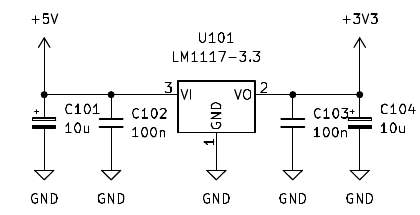
\includegraphics[width = 0.5\textwidth]{LDO.png}
    \caption{Stabilizator napięcia}
    \label{fig:ldo}
\end{figure}


\subsection{Część nadawcza}

\begin{figure}[ht!]
    \centering
    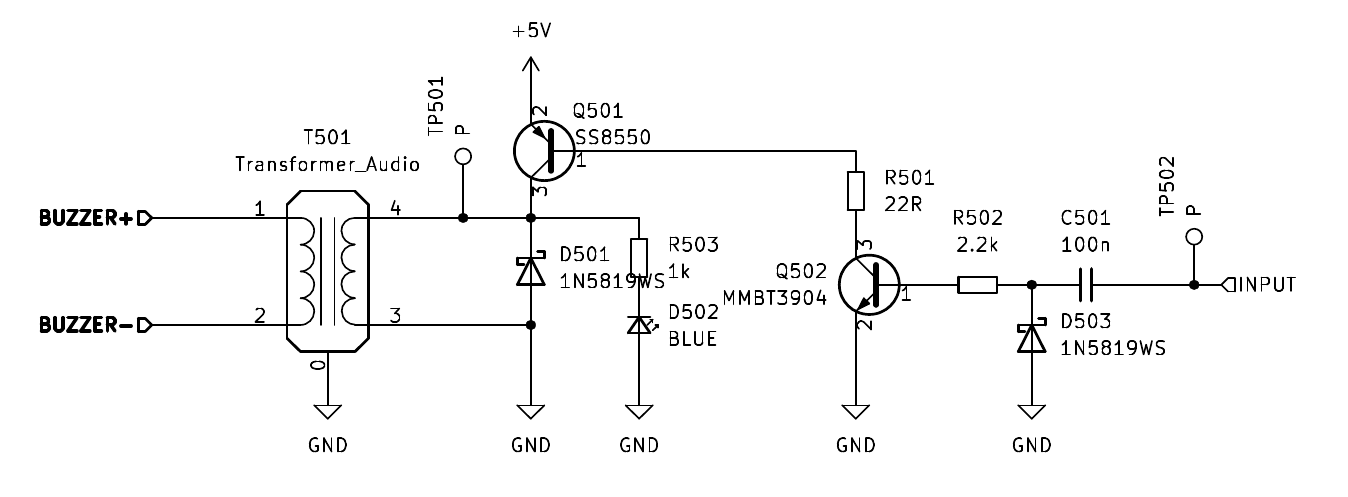
\includegraphics[width = \textwidth]{piezo.png}
    \caption{Wzmacniacz sygnału nadajnika piezoelektrycznego}
    \label{fig:piezo}
\end{figure}

\subsection{Część odbiorcza}
\begin{figure}[ht!]
    \centering
    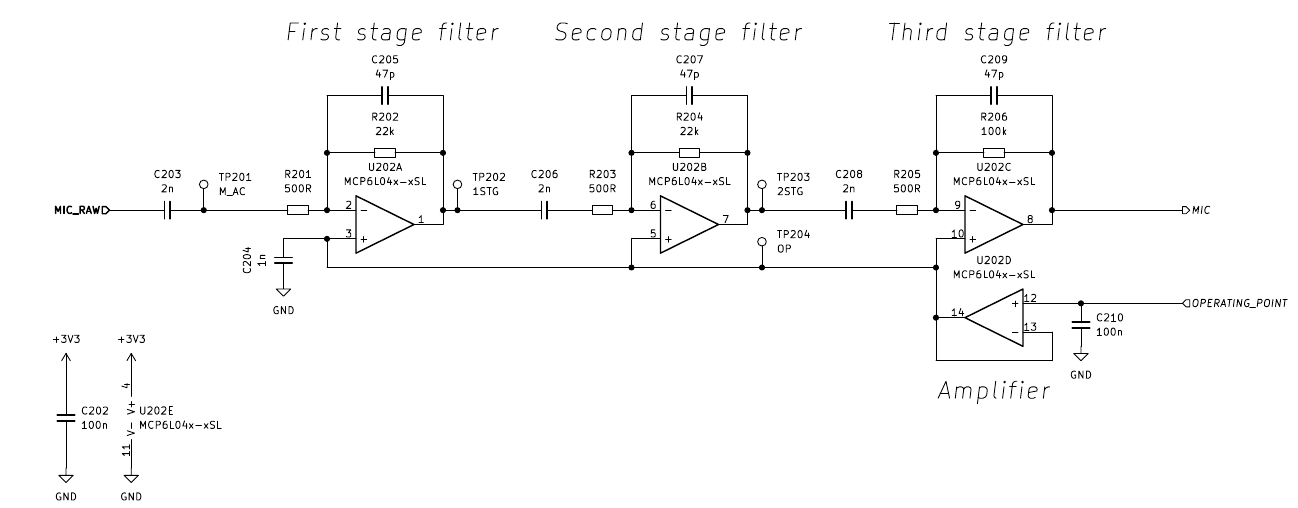
\includegraphics[width = \textwidth]{filter.png}
\end{figure}

\subsection{Symulacja części odbiorczej}
